\documentclass[11pt,a4paper,oneside,openany,indonesian]{report}
\usepackage[a4paper,top=25mm,bottom=25mm,left=30mm,right=25mm,headheight=16pt,headsep=7mm,footskip=12mm]{geometry}
\usepackage{iftex}
\ifLuaTeX
  \usepackage[bidi=basic,shorthands=off,provide=*]{babel}
\else
  \usepackage[bidi=default,shorthands=off,provide=*]{babel}
\fi
\ifPDFTeX\else\babelfont{rm}[]{Charter}\fi
\usepackage{hyperref}
% Shared preamble for the Jakarta TGA chapters.
\usepackage{xcolor}
\usepackage{graphicx}
\usepackage{amsmath,amssymb}
\usepackage{iftex}
\ifPDFTeX
  \usepackage[T1]{fontenc}
  \usepackage[utf8]{inputenc}
  \usepackage{textcomp}
\else
  \usepackage{unicode-math}
  \defaultfontfeatures{Scale=MatchLowercase}
  \defaultfontfeatures[\rmfamily]{Ligatures=TeX,Scale=1}
\fi
\usepackage{lmodern}
\ifPDFTeX\else
  \setmainfont[]{Times New Roman}
  \setsansfont[]{Arial}
  \IfFontExistsTF{Consolas}{\setmonofont[]{Consolas}}{\setmonofont[]{Courier New}}
\fi
\IfFileExists{microtype.sty}{\usepackage{microtype}}{}
\usepackage{longtable,booktabs,array,tabularx,adjustbox,calc}
\usepackage{pdflscape}
\usepackage{caption}
\captionsetup[table]{skip=6pt}
\newcounter{none}
\usepackage{float}
\usepackage{setspace}
\usepackage{ragged2e}
\usepackage{titlesec}
\usepackage{enumitem}
\usepackage{needspace}
\usepackage{fancyhdr}
\usepackage{newunicodechar}
\usepackage{bookmark}
\usepackage{xurl}
\usepackage{csquotes}
\usepackage[backend=biber,style=authoryear,maxcitenames=2,maxbibnames=99,uniquelist=false,uniquename=false]{biblatex}
\DeclareLanguageMapping{indonesian}{english}
\DefineBibliographyStrings{english}{and={dan},andothers={dkk\adddot}}
\DefineBibliographyStrings{indonesian}{and={dan},andothers={dkk\adddot}}
\AtBeginDocument{\renewcommand*{\finalnamedelim}{\addspace dan\space}}
\addbibresource{references.bib}
\DeclareFieldFormat{title}{#1}
\DeclareFieldFormat[article,inbook,incollection,inproceedings,inreference,patent,thesis,unpublished]{title}{#1}
\AtBeginBibliography{\small\setlength{\bibitemsep}{0.15em}}

\newunicodechar{∅}{\ensuremath{\varnothing}}

% Placeholder untuk gambar yang dibuat manual (peta GIS). Ganti dengan \includegraphics setelah berkas target tersedia.
\newcommand{\GambarPlaceholder}[2][7cm]{%
  \fbox{\parbox[c][#1][c]{0.92\linewidth}{\centering\small
    \textbf{PLACEHOLDER GAMBAR}\\[0.6em]#2}}}

\definecolor{Ink}{HTML}{222222}
\definecolor{RuleGray}{HTML}{666666}

\AtBeginDocument{%
  \hypersetup{linkcolor=Ink,citecolor=Ink,urlcolor=Ink,pdfborder={0 0 0}}%
  \urlstyle{same}%
}

\setstretch{1.5}
\setlength{\parindent}{1.1em}
\setlength{\parskip}{0.28em}
\setlength{\emergencystretch}{2.5em}
\clubpenalty=10000
\widowpenalty=10000
\displaywidowpenalty=10000
\raggedbottom

\setlist[itemize]{leftmargin=1.7em,itemsep=0.25em,topsep=0.35em}
\setlist[enumerate]{leftmargin=1.9em,itemsep=0.25em,topsep=0.35em}

\titleformat{\chapter}[display]
  {\normalfont\bfseries\centering\color{Ink}}
  {}{0pt}{\Large\hyphenpenalty=10000\exhyphenpenalty=10000}
\titlespacing*{\chapter}{0pt}{-6pt}{18pt}
\titleformat{\section}{\Needspace{4\baselineskip}\large\bfseries\color{Ink}}{\thesection}{0.7em}{}
\titleformat{\subsection}{\Needspace{3\baselineskip}\normalsize\bfseries\color{Ink}}{\thesubsection}{0.7em}{}
\titleformat{\subsubsection}{\Needspace{3\baselineskip}\normalsize\bfseries\color{Ink}}{\thesubsubsection}{0.7em}{}

\pagestyle{plain}
\fancyhf{}
\fancyfoot[C]{\thepage}
\renewcommand{\headrulewidth}{0pt}
\renewcommand{\footrulewidth}{0pt}
\fancypagestyle{plain}{%
  \fancyhf{}
  \fancyfoot[C]{\thepage}
  \renewcommand{\headrulewidth}{0pt}
}

\renewcommand{\arraystretch}{1.2}
\setlength{\extrarowheight}{1pt}
\setlength{\tabcolsep}{4pt}
\providecommand{\tightlist}{\setlength{\itemsep}{0pt}\setlength{\parskip}{0pt}}
\setlength{\LTpre}{0.5em}
\setlength{\LTpost}{0.8em}
\AtBeginEnvironment{longtable}{\footnotesize\setstretch{1.0}\setlength{\tabcolsep}{3pt}\setlength{\extrarowheight}{1pt}}
\AtBeginEnvironment{table}{\setstretch{1.0}}
\AtBeginEnvironment{figure}{\setstretch{1.0}}
\AtBeginEnvironment{quote}{\small\setlength{\leftskip}{1.2em}\setlength{\rightskip}{1.2em}}

\graphicspath{{figures/}}

\hypersetup{
  pdftitle={Bab 4 Gambaran Umum Lokasi Penelitian},
  pdfauthor={Mahastri Laksita Sam Widita},
  pdflang={id-ID},
  hidelinks
}

\title{\textbf{Borrowed Size atau Agglomeration Shadow?}\\[0.4em]
Analisis Hubungan Integrasi Metropolitan dengan Kematangan Pusat-Pusat Sekunder di Kawasan Aglomerasi Jakarta}
\providecommand{\subtitle}[1]{\gdef\thesubtitle{#1}}
\subtitle{Bab 4 Gambaran Umum Lokasi Penelitian}
\author{Mahastri Laksita Sam Widita\\NIM 22/503065/TK/54947\\[0.5em]
Pembimbing: Rendy Bayu Aditya\\[0.5em]
Program Studi Perencanaan Wilayah dan Kota\\
Departemen Teknik Arsitektur dan Perencanaan\\
Fakultas Teknik\\
Universitas Gadjah Mada}
\date{Kabupaten Sleman, Daerah Istimewa Yogyakarta\\2026}

\makeatletter
\renewcommand{\maketitle}{%
  \begin{titlepage}
    \centering
    {\Large\bfseries TUGAS AKHIR\par}
    \vfill
    {\LARGE\bfseries \@title\par}
    \vspace{1.2cm}
    {\large \thesubtitle\par}
    \vfill
    {\large \@author\par}
    \vfill
    {\large \@date\par}
  \end{titlepage}}
\makeatother

\begin{document}
\maketitle
\tableofcontents
\clearpage
\setcounter{chapter}{3}
\chapter{Gambaran Umum Lokasi Penelitian}

Bab ini menjelaskan wilayah yang menjadi konteks pengukuran dan alasan pemilihan unit analisis. Uraian disusun untuk membantu pembaca membaca hubungan antara Jakarta, kota-kota penyangga, kabupaten dengan perkembangan perkotaan cepat, serta jaringan transportasi yang menghubungkannya. Bab ini tidak menyajikan diagnosis \emph{borrowed size} atau \emph{agglomeration shadow}. Label pusat sekunder yang muncul di sini adalah label kerja untuk audit data; statusnya diuji kembali pada Bab 5.

\section{Posisi Jabodetabek dalam sistem metropolitan}

Jabodetabek merupakan kawasan metropolitan yang terbentuk dari hubungan harian antara Jakarta dan wilayah di sekitarnya. Hubungan itu melampaui batas provinsi dan batas kewenangan satu pemerintah daerah. Jakarta berperan sebagai inti dengan konsentrasi fungsi pemerintahan, jasa tingkat tinggi, kegiatan ekonomi, dan simpul transportasi. Bogor, Depok, Tangerang, dan Bekasi menampung perumahan, pekerjaan, industri, pendidikan, perdagangan, serta fasilitas yang tumbuh dengan tingkat kemandirian yang berbeda. Kabupaten di sekeliling kota tersebut juga memuat kawasan industri, perumahan baru, lahan pertanian yang tersisa, dan jaringan jalan antarkota.

Pilihan Jabodetabek sebagai kasus memberi kesempatan untuk menguji pertanyaan penelitian dalam satu sistem yang memiliki inti dominan, beberapa kota besar, dan hubungan lintas batas yang terdokumentasi. Literatur tentang perkembangan Jabotabek mencatat perluasan permukiman sekaligus perubahan struktur pekerjaan, industri, jaringan, dan hubungan antarsubwilayah \parencite{henderson1996,hudalahfirman2012,hudalahetal2013}. Penelitian yang lebih baru juga menemukan bahwa jarak ke pusat dan status administratif belum cukup untuk menjelaskan hubungan antarsuburban \parencite{sadewoetal2023,aritenang2023}. Karena itu, lokasi penelitian diperlakukan sebagai sistem relasional, sedangkan administrasi dipakai sebagai unit pembacaan dan pelaporan.

Laporan JUTPI 3 menggambarkan Jabodetabek sebagai wilayah kebijakan transportasi yang membutuhkan koordinasi lintas pemerintah. Laporan tersebut memuat Bogor, Depok, Tangerang, dan Bekasi bersama Jakarta dalam struktur pelaksanaan dan pembahasan jaringan transportasi \parencite{jica2025jutpi}. Hal ini membantu menetapkan cakupan geografis penelitian, tetapi tidak otomatis menjadikan setiap rencana jaringan sebagai kondisi aktual. Rencana jaringan, jaringan yang beroperasi, dan arus perjalanan aktual dipisahkan pada tahap audit bukti.

\section{Wilayah administratif dan batas penelitian}

Wilayah utama penelitian menggunakan sembilan satuan administratif berikut: DKI Jakarta, Kabupaten Bogor, Kota Bogor, Kota Depok, Kabupaten Tangerang, Kota Tangerang, Kota Tangerang Selatan, Kabupaten Bekasi, dan Kota Bekasi. DKI Jakarta diperlakukan sebagai satu bagian inti pada analisis metropolitan, meskipun geometri administrasinya terdiri atas lima kota administrasi dan satu kabupaten administrasi. Pemecahan internal DKI digunakan jika indikator hanya tersedia pada tingkat kota administrasi.

Batas geografis pada peta kerja diambil dari geometri ADM2 geoBoundaries untuk Indonesia. Geometri tersebut menyediakan poligon yang konsisten untuk kebutuhan visualisasi awal, tetapi merupakan geometri yang disederhanakan. Geometri tidak digunakan untuk menetapkan daerah tangkapan, pusat pelayanan, atau batas fungsional. Perbedaan tahun antara geometri, data penduduk, data jaringan, dan data lokasi usaha ditangani pada audit temporal Bab 3 dan tidak disamarkan sebagai panel tahunan yang lengkap.

\begin{figure}[H]
  \centering
  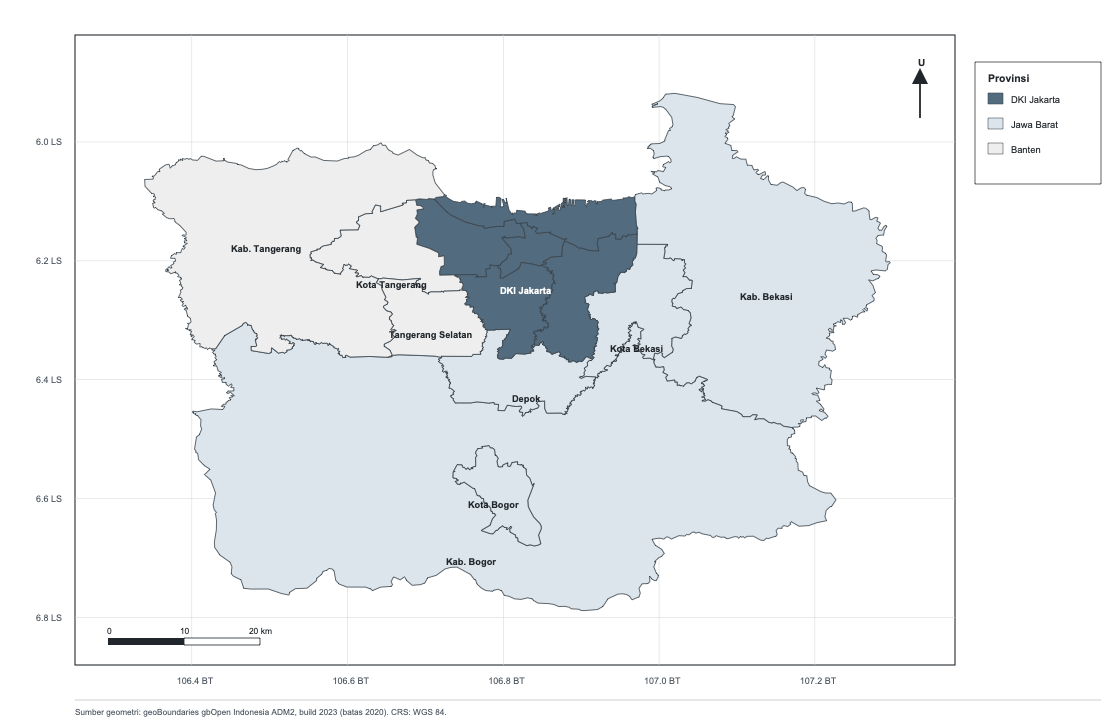
\includegraphics[width=0.98\textwidth]{bab4_admin.png}
  \caption{Batas administratif wilayah penelitian. Sumber: geoBoundaries gbOpen Indonesia ADM2, build 2023 dengan geometri yang merepresentasikan batas administratif tahun 2020; diunduh 19 September 2026. Proyeksi visual WGS84 geografis. Skala dan orientasi digunakan untuk pembacaan konteks.}
  \label{fig:bab4-admin}
\end{figure}

Gambar \ref{fig:bab4-admin} memperlihatkan posisi relatif sembilan unit dan menjadi peta batas tetap untuk pelaporan. Hubungan ekonomi, perjalanan, dan pelayanan dapat melintasi garis tersebut. Batas administrasi digunakan untuk menempatkan hasil pada kewenangan yang sesuai.

\begin{figure}[H]
  \centering
  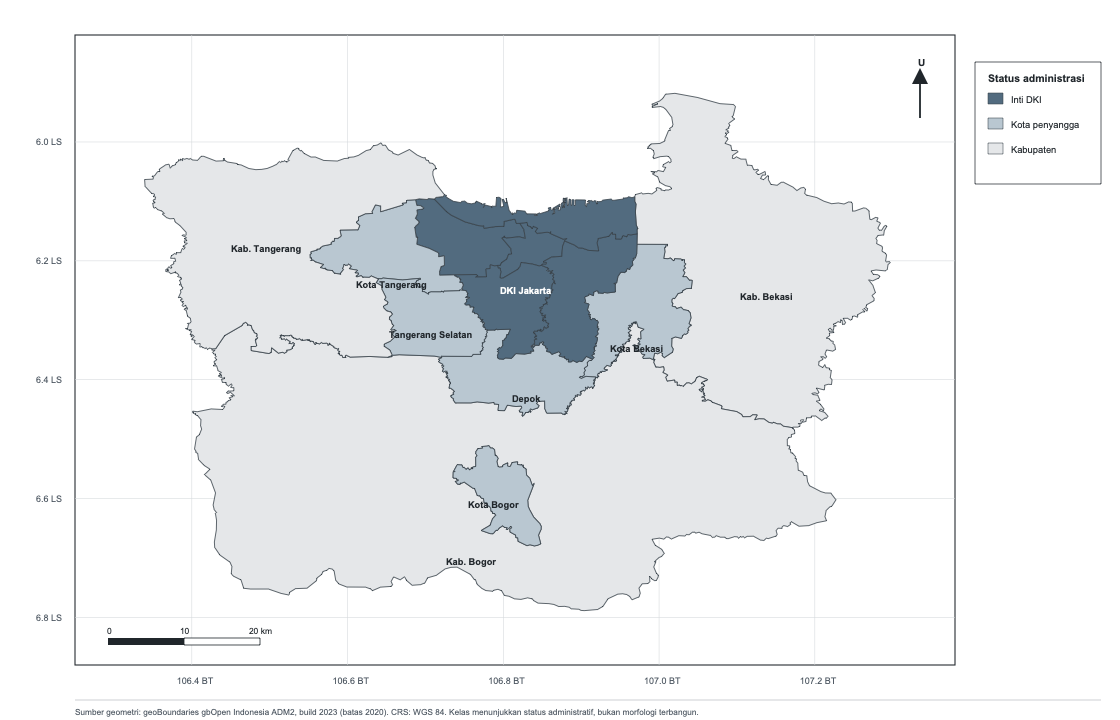
\includegraphics[width=0.98\textwidth]{bab4_status_administratif.png}
  \caption{Status administratif wilayah penelitian. Sumber geometri: geoBoundaries gbOpen Indonesia ADM2, build 2023 dengan batas tahun 2020. Kelas membedakan inti DKI, kota penyangga, dan kabupaten untuk kebutuhan pelaporan; kelas tersebut bukan ukuran morfologi terbangun atau kematangan pusat.}
  \label{fig:bab4-status-administratif}
\end{figure}

Gambar \ref{fig:bab4-status-administratif} membedakan status administrasi yang akan digunakan sebagai kondisi kontekstual. Kota dan kabupaten memiliki luas, kepadatan, kewenangan, serta komposisi wilayah yang berbeda. Perbedaan tersebut perlu diperiksa ketika hasil antarpusat dibandingkan, tetapi status kota tidak dengan sendirinya menetapkan suatu unit sebagai pusat sekunder.

\subsection{Cakupan wilayah dan aturan pembacaan}

Cakupan studi dipilih agar pusat inti dan wilayah penyangga utama dapat dibaca dalam satu kerangka. Kabupaten Bogor dan Kabupaten Bekasi berukuran luas dan memiliki kombinasi wilayah perkotaan, industri, serta perdesaan. Kabupaten Tangerang juga memuat koridor urban yang berbeda dari Kota Tangerang dan Kota Tangerang Selatan. Kota Bogor, Kota Depok, Kota Bekasi, Kota Tangerang, dan Kota Tangerang Selatan diperlakukan sebagai unit kota yang dapat memiliki massa lokal dan fungsi relatif sendiri.

Aturan pembacaannya adalah sebagai berikut. Pertama, angka penduduk dibaca sebagai massa lokal, bukan sebagai ukuran lengkap kapasitas pusat. Kedua, lokasi usaha, fasilitas, bangunan, jaringan, dan informasi operator diperlakukan sebagai sumber observasi yang dapat memiliki bias cakupan. Ketiga, hasil estimasi pekerjaan atau perjalanan tidak disamakan dengan pencatatan administratif. Keempat, peta kerja tidak dapat digunakan untuk menyimpulkan pusat sekunder sebelum indikator fungsi, integrasi, manfaat, dan beban diuji.

\section{Demografi dan massa lokal}

Massa lokal diperlukan sebagai tolok ukur ketika penelitian membandingkan fungsi pusat dengan ukuran wilayahnya. Untuk menjaga keterbandingan, Bab ini menggunakan proyeksi penduduk 2024 yang dipublikasikan BPS untuk unit di Jawa Barat dan Banten. Angka di bawah ditulis dalam ribu jiwa dan mengikuti definisi proyeksi pada publikasi asal. Perbedaan basis antara proyeksi, sensus, dan pencacahan administratif tetap dicatat sebagai sumber ketidakpastian.

\begin{table}[H]
\centering
\caption{Massa penduduk unit non-DKI dalam wilayah penelitian, 2024}
\label{tab:bab4-populasi}
\begin{tabularx}{\textwidth}{>{\raggedright\arraybackslash}p{0.38\textwidth} >{\raggedleft\arraybackslash}p{0.20\textwidth} >{\raggedright\arraybackslash}X}
\toprule
Unit administratif & Penduduk (ribu jiwa) & Sumber dan batas pembacaan \\
\midrule
Kabupaten Bogor & 5.682,30 & Proyeksi 2024 BPS Jawa Barat; kabupaten, bukan aglomerasi fungsional. \\
Kota Bogor & 1.078,35 & Proyeksi 2024 BPS Jawa Barat; kota administratif. \\
Kota Depok & 2.163,64 & Proyeksi 2024 BPS Jawa Barat; kota administratif. \\
Kabupaten Bekasi & 3.273,87 & Proyeksi 2024 BPS Jawa Barat; kabupaten. \\
Kota Bekasi & 2.644,06 & Proyeksi 2024 BPS Jawa Barat; kota administratif. \\
Kabupaten Tangerang & 3.400,49 & Proyeksi 2024 BPS Banten; kabupaten. \\
Kota Tangerang & 1.963,97 & Proyeksi 2024 BPS Banten; kota administratif. \\
Kota Tangerang Selatan & 1.399,50 & Proyeksi 2024 BPS Banten; kota administratif. \\
\bottomrule
\end{tabularx}
\smallskip
\parbox{\textwidth}{\footnotesize Catatan: angka Jawa Barat diambil dari tabel perbandingan kabupaten/kota pada \emph{Kota Depok Dalam Angka 2025}; angka Banten diambil dari tabel perbandingan kabupaten/kota pada \emph{Kota Tangerang Dalam Angka 2024}. Satuan, tahun, dan cakupan mengikuti sumber masing-masing \parencite{bpsjabar2025,bpsbanten2024}. Angka DKI tidak dijumlahkan ulang di tabel ini karena publikasi DKI memecahnya pada kota administrasi dan menggunakan tabel sektoral yang berbeda; rujukan auditnya adalah \emph{Provinsi DKI Jakarta Dalam Angka 2025} \parencite{bpsdki2025}.}
\end{table}

Tabel \ref{tab:bab4-populasi} menunjukkan massa lokal yang besar di beberapa wilayah luar DKI, terutama Kabupaten Bogor, Kabupaten Tangerang, Kabupaten Bekasi, Kota Bekasi, dan Kota Depok. Angka tersebut belum menunjukkan bahwa unit-unit itu memiliki fungsi metropolitan yang setara dengan Jakarta. Dalam analisis berikutnya, jumlah penduduk menjadi pembagi awal untuk menilai apakah fungsi yang teramati atau diperkirakan sebanding dengan massa lokalnya.

Perbedaan massa lokal juga penting bagi interpretasi hasil. Pusat dengan penduduk besar dapat memiliki fungsi yang tampak tinggi secara absolut tetapi biasa saja setelah dibandingkan dengan ukurannya. Sebaliknya, pusat dengan penduduk lebih kecil dapat menunjukkan fungsi khusus atau akses ke jaringan metropolitan tanpa memiliki jumlah fasilitas terbesar. Perbandingan relatif pada Bab 5 karena itu akan menggunakan indikator dengan unit dan tahun yang dijelaskan, serta menyertakan pemeriksaan sensitivitas terhadap pilihan pembagi.

\section{Morfologi terbangun dan jaringan transportasi}

Morfologi Jabodetabek terbentuk dari gabungan inti perkotaan padat, koridor jalan dan rel, kawasan industri, perumahan berskala besar, serta ruang terbuka yang tersisa di antara kawasan terbangun. Bentuk tersebut berubah melalui perluasan kawasan industri dan perumahan, pembangunan jalan tol dan jalan arteri, penguatan jaringan rel, serta pertumbuhan pusat perdagangan dan jasa. Studi tentang dekonsentrasi manufaktur dan transformasi pascasuburban menunjukkan bahwa perkembangan tersebut berlangsung tidak seragam antarwilayah \parencite{hudalahetal2013,hudalahfirman2012}.

Peta morfologi baru disusun setelah jejak bangunan atau raster tutupan terbangun lolos audit tahun, resolusi, klasifikasi, lisensi, dan cakupan. Naskah ini tidak memakai kelas administratif pada Gambar \ref{fig:bab4-status-administratif} sebagai pengganti morfologi. Jika lapisan yang lolos audit hanya tersedia untuk satu periode, hasilnya menjadi potret morfologi pada periode tersebut. Perubahan hanya dihitung apabila produk dan definisinya dapat disejajarkan.

Jaringan transportasi memberi jalur yang memungkinkan hubungan metropolitan terbentuk, tetapi keberadaan jaringan tidak sama dengan penggunaan. Laporan JUTPI 3 membahas jaringan publik masa depan dengan horizon 2045 dan menampilkan MRT, LRT, KCI, BRT, dan trem dalam peta usulan \parencite{jica2025jutpi}. Peta itu berguna untuk membaca arah kebijakan dan kemungkinan konektivitas, sedangkan analisis penelitian memerlukan pembedaan antara jaringan yang sudah beroperasi, jaringan yang direncanakan, frekuensi layanan, kapasitas, dan arus penumpang.

\begin{figure}[H]
  \centering
  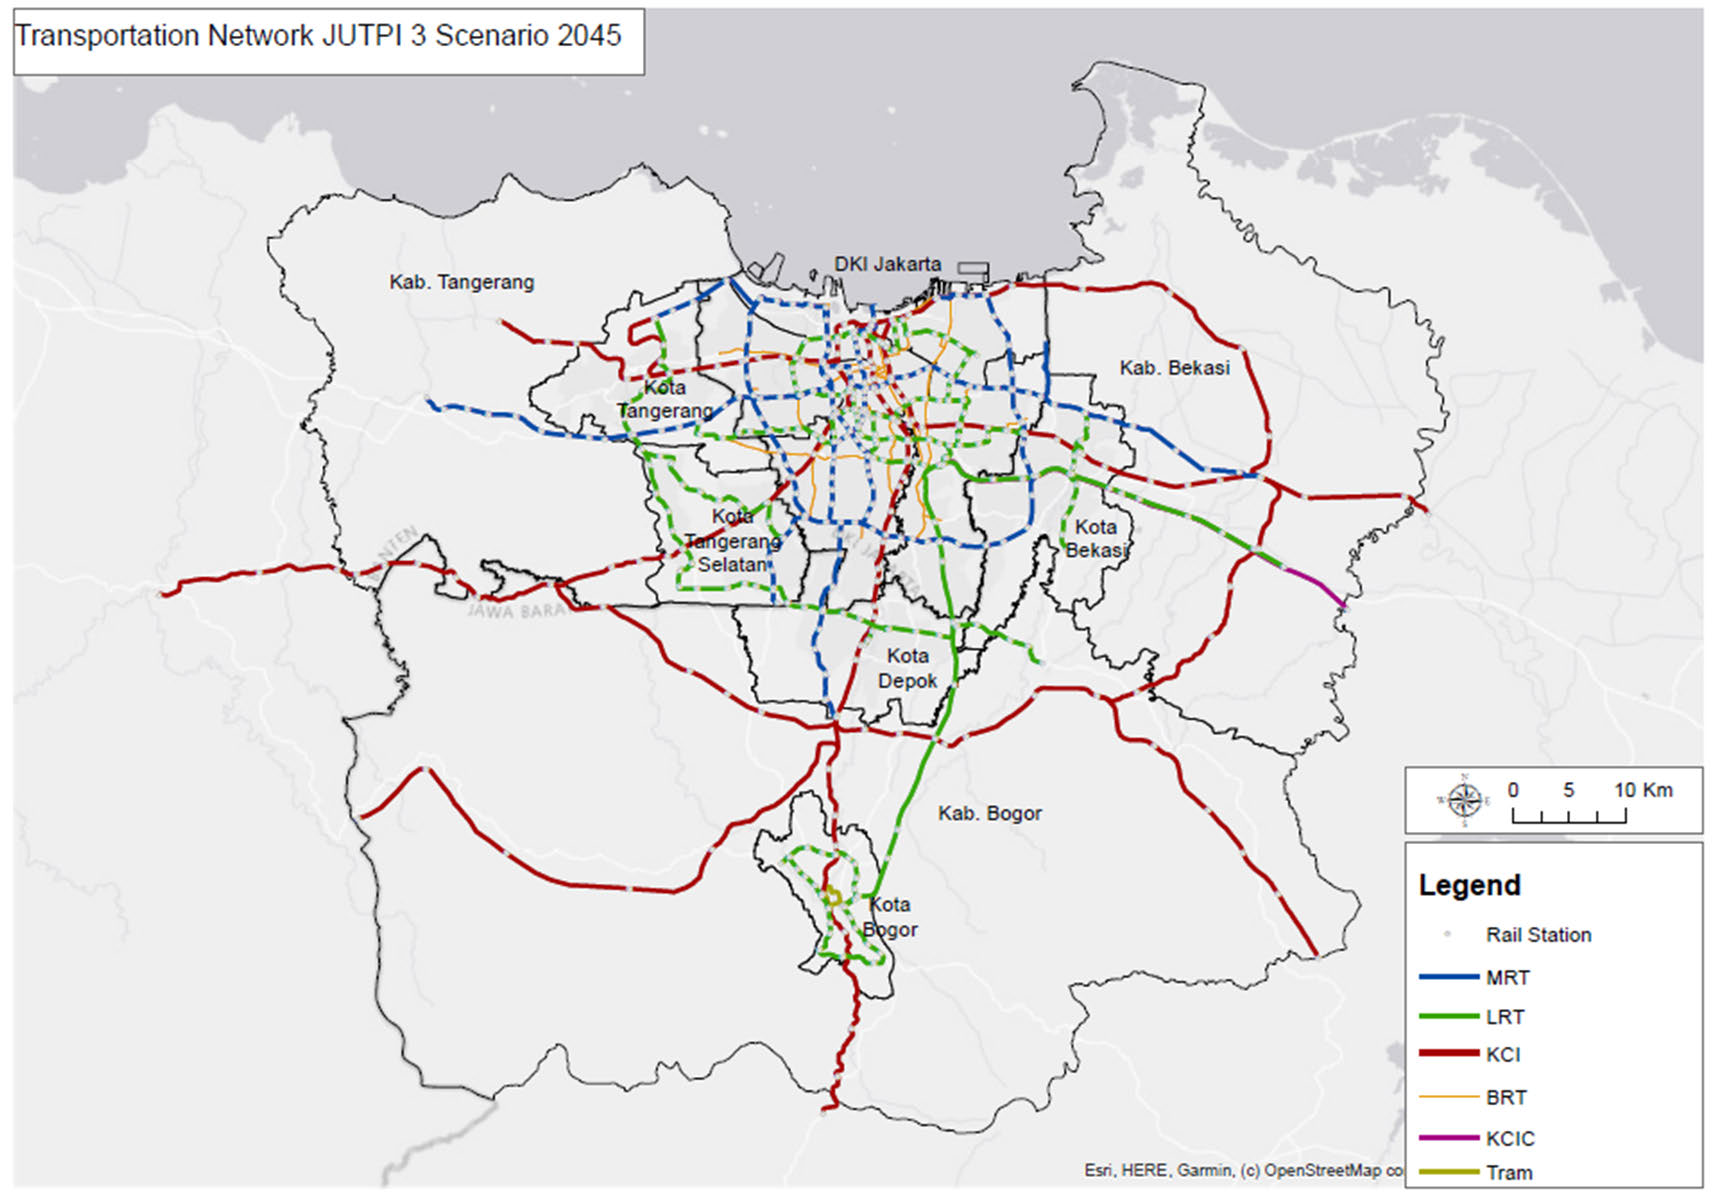
\includegraphics[width=0.90\textwidth]{bab4_network_jutpi.png}
  \caption{Peta jaringan angkutan umum masa depan yang diusulkan JUTPI 3 untuk Jabodetabek. Sumber: JICA Expert Team dalam \emph{Project Completion Report} 2025. Peta dibaca sebagai skenario kebijakan dan konteks jaringan, bukan pengamatan arus perjalanan aktual.}
  \label{fig:bab4-network}
\end{figure}

Peta jaringan JUTPI 3 memperlihatkan mengapa integrasi metropolitan tidak tepat direduksi menjadi kedekatan geometris. Hubungan antarwilayah dibentuk oleh simpul, koridor, waktu tempuh, kapasitas, pertukaran moda, dan hambatan perjalanan. Variabel jaringan aktual pada Bab 5 dipilih setelah audit terhadap data operator dan sumber terbuka. Rekaman CCTV yang tersedia dapat diolah dengan deteksi YOLO, pelacakan objek, dan garis hitung untuk mengestimasi arus pada titik serta waktu tertentu. SUMO digunakan hanya jika jaringan, permintaan, dan data kalibrasinya memadai.

\section{Industri, pusat pelayanan, dan aktivitas ekonomi}

Kawasan industri di Bekasi, Tangerang, dan sebagian Bogor merupakan konteks penting untuk membaca kemungkinan perubahan hubungan pekerjaan dan perjalanan. Penelitian sebelumnya mendokumentasikan perpindahan sebagian kegiatan manufaktur dari inti Jakarta ke kawasan metropolitan dan munculnya pola kerja antarsuburban \parencite{hudalahetal2013,permatasarihudalah2013,sadewoetal2023}. Namun, keberadaan kawasan industri tidak menunjukkan jumlah pekerjaan yang sedang tersedia pada tahun tertentu. Luas lahan, daftar perusahaan, lokasi gerbang, dan informasi operator harus dibedakan dari pekerjaan aktual.

Pusat pelayanan juga memiliki beberapa tingkat. Rumah sakit rujukan, kampus, pusat perdagangan, kantor pemerintahan, ruang budaya, dan fasilitas rekreasi dapat melayani penduduk lokal atau menarik pengguna dari wilayah lain. Lokasi fasilitas dari situs pemerintah, OpenStreetMap, dan direktori usaha dapat dipakai untuk membentuk observasi titik. Atribut seperti kapasitas, tingkat layanan, jam operasi, dan status aktif harus dicatat jika tersedia. Ketika atribut tidak tersedia, titik hanya dibaca sebagai indikasi keberadaan, bukan ukuran kualitas atau volume pengguna.

Sumber lokasi usaha seperti Google Maps, OpenStreetMap, data pemerintah daerah, dan situs operator dapat saling melengkapi. Setiap sumber memiliki mekanisme cakupan, pembaruan, dan duplikasi yang berbeda. Prosedur deduplikasi, pemeriksaan sampel manual, geocoding, dan pencatatan tanggal akses menjadi bagian dari audit. Keluaran akhirnya membedakan tiga status: observasi yang langsung terlihat pada sumber, estimasi yang dihitung dari observasi dengan asumsi, dan simulasi yang menggambarkan skenario.

\section{Kandidat pusat sekunder dan hubungan transportasi}

Penelitian tidak menetapkan pusat sekunder hanya karena sebuah wilayah berstatus kota atau memiliki penduduk besar. Label kerja digunakan untuk memeriksa beberapa lokasi yang secara awal memiliki kombinasi massa lokal, aktivitas, jaringan, dan potensi fungsi relatif. Label tersebut dapat berubah setelah data dibersihkan dan indikator diuji.

\begin{figure}[H]
  \centering
  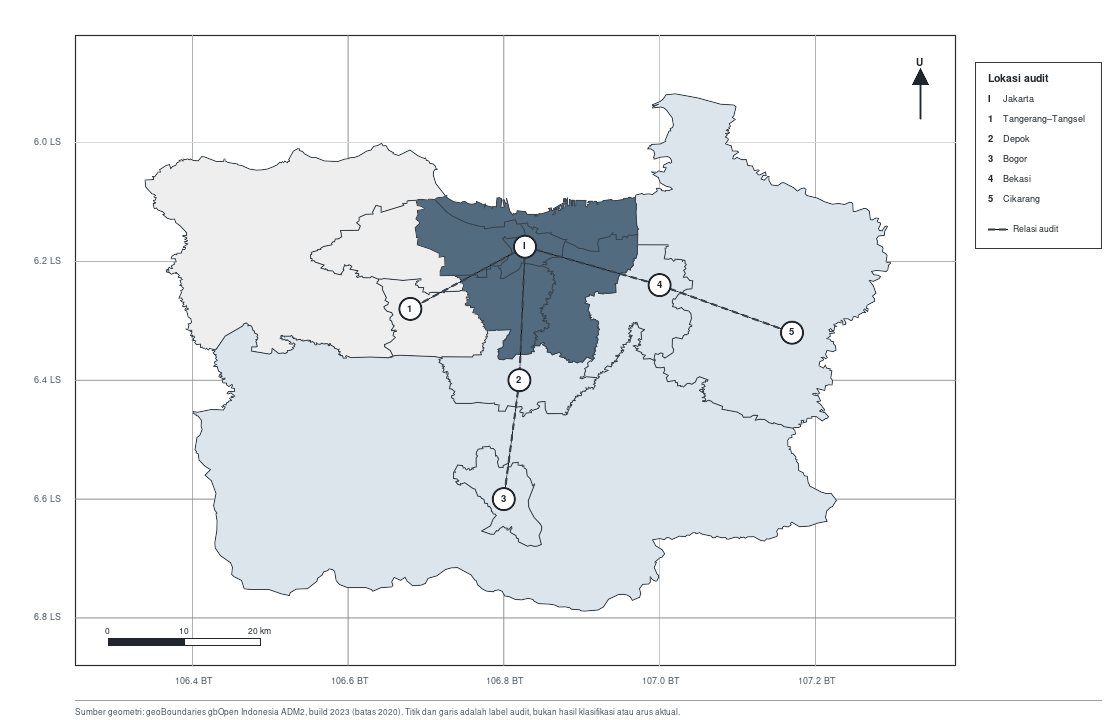
\includegraphics[width=0.98\textwidth]{bab4_candidates.png}
  \caption{Kandidat pusat sekunder sebagai label operasional awal. Nomor menunjukkan lokasi kerja dan garis putus-putus menunjukkan pasangan relasi yang perlu diaudit, bukan hasil klasifikasi atau arus perjalanan aktual. Sumber geometri: geoBoundaries gbOpen Indonesia ADM2; proyeksi visual WGS84 geografis dengan skala dan orientasi.}
  \label{fig:bab4-candidates}
\end{figure}

Gambar \ref{fig:bab4-candidates} menempatkan Jakarta inti, Tangerang dan Tangerang Selatan, Depok, Bogor, Bekasi, serta Cikarang sebagai titik audit awal. Cikarang berada dalam Kabupaten Bekasi dan dipisahkan sebagai lokasi kerja karena konteks industri dan jaringan dapat berbeda dari rata-rata kabupaten. Pemisahan tersebut belum berarti bahwa Cikarang akan menjadi pusat sekunder dalam hasil akhir. Unit analisis dapat berupa kota, kabupaten, koridor, atau klaster titik jika bukti dan tujuan pengukuran mengharuskannya.

Hubungan transportasi dan komuter dipakai untuk membaca hubungan fungsional. Survei Komuter Jabodetabek 2023 dari BPS menjadi rujukan terbuka untuk definisi dan tabulasi komuter, sementara laporan operator, berita resmi, dan data jaringan dapat digunakan untuk memeriksa layanan pada periode lain. Data perjalanan aktual tidak disimpulkan dari peta rencana. Jika data asal-tujuan terbuka tersedia, arus tersebut dilaporkan sebagai observasi. Jika hanya kapasitas armada, frekuensi, atau jumlah perjalanan yang tersedia, informasi tersebut digunakan sebagai batas atas, indikator kapasitas, atau bahan estimasi dengan asumsi yang ditulis.

Penggunaan CCTV dan SUMO ditempatkan sebagai penguatan bersyarat. Hitungan dari rekaman CCTV harus diuji pada sampel manual yang mewakili perbedaan kamera, kepadatan, cuaca, pencahayaan, sudut pandang, dan oklusi. Hasilnya dilaporkan sebagai estimasi menurut kamera, waktu, arah, dan kelas objek. Hitungan tersebut bukan matriks asal dan tujuan. SUMO dapat digunakan untuk simulasi skenario ketika jaringan, permintaan, dan parameter kalibrasi tersedia. Hasil simulasi tidak disebut arus aktual dan tidak menggantikan observasi.

\section{Audit sumber dan periode}

Audit sumber pada Tabel \ref{tab:bab4-audit} menjadi penghubung antara gambaran lokasi dan metode pengukuran. Tahun pada tabel adalah tahun observasi, tahun proyeksi, tahun geometri, atau tahun publikasi sesuai keterangan. Satu baris tidak boleh dipakai untuk menyiratkan seri waktu yang tidak ada.

\begingroup
\footnotesize
\setlength{\tabcolsep}{4pt}
\begin{longtable}{>{\raggedright\arraybackslash}p{0.19\textwidth} >{\raggedright\arraybackslash}p{0.17\textwidth} >{\raggedright\arraybackslash}p{0.15\textwidth} >{\raggedright\arraybackslash}p{0.41\textwidth}}
\caption{Audit sumber terbuka dan periode untuk Bab 4}\label{tab:bab4-audit}\\
\toprule
Konstruk/lapisan & Sumber & Tahun/periode & Status bukti dan batas penggunaan \\
\midrule
\endfirsthead
\caption[]{Audit sumber terbuka dan periode untuk Bab 4 (lanjutan)}\\
\toprule
Konstruk/lapisan & Sumber & Tahun/periode & Status bukti dan batas penggunaan \\
\midrule
\endhead
\midrule
\multicolumn{4}{r}{\footnotesize Dilanjutkan pada halaman berikutnya}\\
\endfoot
\bottomrule
\endlastfoot
Batas administratif & geoBoundaries gbOpen ADM2 & build 2023; geometri 2020 & Observasi geometri konteks. Tidak menetapkan batas fungsional atau daerah tangkapan \parencite{geoboundaries2023}. \\
Massa penduduk Jawa Barat & BPS, tabel kabupaten/kota dalam \emph{Kota Depok Dalam Angka 2025} & Proyeksi 2021--2025; digunakan 2024 & Angka proyeksi dalam ribu jiwa; unit kabupaten/kota. \\
Massa penduduk Banten & BPS, tabel kabupaten/kota dalam \emph{Kota Tangerang Dalam Angka 2024} & Proyeksi 2020--2024; digunakan 2024 & Angka proyeksi dalam ribu jiwa; unit kabupaten/kota. \\
Statistik DKI & BPS Provinsi DKI Jakarta, \emph{Provinsi DKI Jakarta Dalam Angka 2025} & Publikasi 2025; indikator sektoral bervariasi & Sumber audit untuk kota administrasi, demografi, ekonomi, dan layanan; angka dipakai bersama tahun indikator. \\
Jaringan dan skenario transportasi & JICA Expert Team, JUTPI 3 & Laporan 2025; jaringan usulan 2045 & Skenario dan konteks kebijakan. Tidak dibaca sebagai jaringan aktual atau arus aktual \parencite{jica2025jutpi}. \\
Komuter & BPS, Survei Komuter Jabodetabek & 2023 & Definisi dan tabulasi komuter. Cakupan, unit, dan tabel yang dipakai dicatat kembali pada manifest data. \\
Bangunan dan tutupan terbangun & sumber raster atau jejak bangunan terbuka yang lolos audit & periode mengikuti produk & Akan dipakai hanya jika tahun, resolusi, lisensi, dan metode ekstraksi dapat ditelusuri. \\
Lokasi usaha dan fasilitas & pemerintah daerah, OpenStreetMap, direktori usaha, dan situs operator & tanggal akses per ekstraksi & Observasi titik dengan bias cakupan. Deduplikasi dan pemeriksaan sampel wajib dicatat. \\
Rekaman lalu lintas titik & Rekaman CCTV yang telah tersedia & Periode mengikuti metadata setiap rekaman; belum diaudit & Video merupakan observasi mentah. Hitungan YOLO dan pelacakan objek berstatus estimasi turunan serta memerlukan validasi manual menurut kamera, waktu, arah, dan kelas objek. \\
Kandidat pusat & gabungan lapisan terbuka dan literatur & label awal Bab 4 & Status operasional; bukan hasil klasifikasi dan tidak menjadi bukti tunggal fungsi. \\
\end{longtable}
\endgroup

Tabel tersebut sengaja memisahkan sumber yang sudah memiliki angka dari sumber yang baru menjadi rujukan konteks. Peta JUTPI 3, misalnya, dapat memperlihatkan arah jaringan dan lokasi simpul yang direncanakan, tetapi tidak dapat dipakai untuk menghitung integrasi aktual tanpa data operasi. Demikian pula, direktori usaha dapat membantu menemukan lokasi dan perubahan keberadaan, tetapi tidak langsung mengukur omzet, jumlah pekerja, atau jumlah pengunjung.

\section{Batas interpretasi gambaran lokasi}

Bab 4 menyediakan batas administratif tetap untuk pemetaan antarsumber, gambaran massa lokal dan struktur wilayah untuk membaca perbedaan antarpusat, serta daftar titik dan lapisan terbuka yang akan diaudit dan diuji sensitivitasnya. Ketiganya menjadi konteks bagi pengukuran, bukan hasil diagnosis.

Bab ini tidak mengklaim bahwa semua indikator sudah memiliki rentang tahun yang sama. Seri waktu hanya dibentuk untuk indikator yang memiliki definisi, unit, dan cakupan yang dapat disejajarkan. Indikator dengan satu tahun atau periode berbeda tetap dapat digunakan sebagai konteks atau potret, dengan statusnya ditulis. Jika audit berikutnya menemukan bahwa satu sumber tidak cukup stabil, indikator tersebut diturunkan menjadi hasil estimasi atau dikeluarkan dari konstruksi inti tanpa mengubah arah penelitian.

Dengan aturan ini, istilah pusat sekunder berarti kandidat unit yang akan diuji terhadap fungsi relatif, integrasi, manfaat, beban, dan hubungan metropolitan. Istilah tersebut belum merupakan kesimpulan. Bab 5 menjadi tempat untuk menunjukkan apakah pola yang terukur lebih dekat dengan manfaat yang dipinjam, bayangan aglomerasi, campuran keduanya, atau hasil yang belum terselesaikan pada konstruk tertentu.

\printbibliography[heading=bibintoc,title={Daftar Pustaka}]
\end{document}
